\begin{figure}[tbp]
\centering
\begingroup
\newcommand{\FiniteSquare}[3]{%
  \begin{scope}[shift={(#1,#2)}]
    \draw[finite boundary] (-.35,-.35) rectangle (.35,.35);
    #3
    \foreach \p in {(-.35,0),(0,-.35),(.35,0),(0,.35)}
      \fill[black!45] \p circle (1pt);
  \end{scope}}
\newcommand{\FiniteTriangle}[3]{%
  \begin{scope}[shift={(#1,#2)}]
    \draw[finite boundary] (-.48,-.33)--(.48,-.33)--(0,.51)--cycle;
    #3
    \foreach \p in {(0,-.33),(-.24,.09),(.24,.09)}
      \fill[black!45] \p circle (1pt);
  \end{scope}}
\newcommand{\FiniteCap}[3]{%
  \begin{scope}[shift={(#1,#2)}]
    \draw[finite boundary] (-.48,.22)--(-.48,-.35)--(.48,-.35)--(.48,.22);
    #3
    \foreach \p in {(-.30,.22),(.30,.22)}
      \fill[black!45] \p circle (1pt);
  \end{scope}}
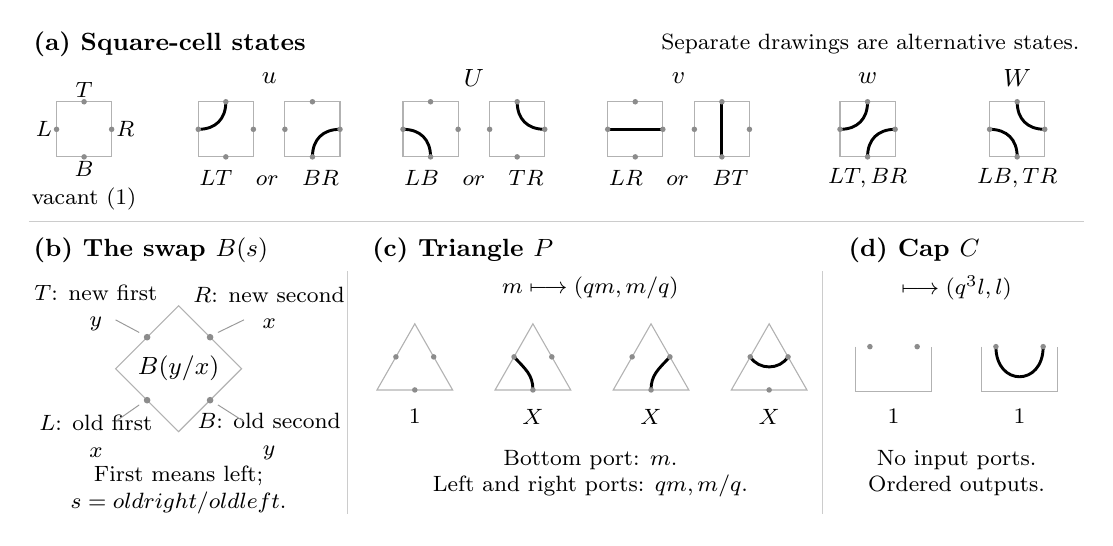
\begin{tikzpicture}[
  x=1cm,y=1cm,
  font=\small,
  finite boundary/.style={draw=black!30,line width=.4pt},
  finite arc/.style={draw=black,line width=1.05pt,line cap=round},
  every node/.style={inner sep=1.5pt},
  finite label/.style={font=\footnotesize},
  finite heading/.style={anchor=west,font=\small\bfseries}
]
  \node[finite heading] at (0,0) {(a) Square-cell states};
  \node[anchor=east,font=\footnotesize] at (13.4,0)
    {Separate drawings are alternative states.};

  \FiniteSquare{.70}{-1.08}{}
  \node[finite label,left]  at (.35,-1.08) {$L$};
  \node[finite label,below] at (.70,-1.43) {$B$};
  \node[finite label,right] at (1.05,-1.08) {$R$};
  \node[finite label,above] at (.70,-.73) {$T$};
  \node[finite label] at (.70,-1.96) {vacant ($1$)};

  \node at (3.05,-.43) {$u$};
  \FiniteSquare{2.50}{-1.08}{%
    \draw[finite arc] (-.35,0) .. controls (-.13,0) and (0,.13) .. (0,.35);}
  \FiniteSquare{3.60}{-1.08}{%
    \draw[finite arc] (0,-.35) .. controls (0,-.13) and (.13,0) .. (.35,0);}
  \node[finite label] at (3.05,-1.70) {$LT\quad\text{or}\quad BR$};

  \node at (5.65,-.43) {$U$};
  \FiniteSquare{5.10}{-1.08}{%
    \draw[finite arc] (-.35,0) .. controls (-.13,0) and (0,-.13) .. (0,-.35);}
  \FiniteSquare{6.20}{-1.08}{%
    \draw[finite arc] (0,.35) .. controls (0,.13) and (.13,0) .. (.35,0);}
  \node[finite label] at (5.65,-1.70) {$LB\quad\text{or}\quad TR$};

  \node at (8.25,-.43) {$v$};
  \FiniteSquare{7.70}{-1.08}{\draw[finite arc] (-.35,0)--(.35,0);}
  \FiniteSquare{8.80}{-1.08}{\draw[finite arc] (0,-.35)--(0,.35);}
  \node[finite label] at (8.25,-1.70) {$LR\quad\text{or}\quad BT$};

  \node at (10.65,-.43) {$w$};
  \FiniteSquare{10.65}{-1.08}{%
    \draw[finite arc] (-.35,0) .. controls (-.13,0) and (0,.13) .. (0,.35);
    \draw[finite arc] (0,-.35) .. controls (0,-.13) and (.13,0) .. (.35,0);}
  \node[finite label] at (10.65,-1.70) {$LT,BR$};

  \node at (12.55,-.43) {$W$};
  \FiniteSquare{12.55}{-1.08}{%
    \draw[finite arc] (-.35,0) .. controls (-.13,0) and (0,-.13) .. (0,-.35);
    \draw[finite arc] (0,.35) .. controls (0,.13) and (.13,0) .. (.35,0);}
  \node[finite label] at (12.55,-1.70) {$LB,TR$};

  \draw[black!20] (0,-2.25)--(13.4,-2.25);
  \node[finite heading] at (0,-2.62) {(b) The swap $B(s)$};
  \node[finite heading] at (4.30,-2.62) {(c) Triangle $P$};
  \node[finite heading] at (10.35,-2.62) {(d) Cap $C$};

  \draw[finite boundary] (1.90,-3.32)--(2.70,-4.12)--(1.90,-4.92)--(1.10,-4.12)--cycle;
  \node at (1.90,-4.12) {$B(y/x)$};
  \foreach \p in {(1.50,-3.72),(2.30,-3.72),(1.50,-4.52),(2.30,-4.52)}
    \fill[black!45] \p circle (1.2pt);
  \node[finite label,align=center] at (.85,-3.35) {$T$: new first\\$y$};
  \node[finite label,align=center] at (3.05,-3.35) {$R$: new second\\$x$};
  \node[finite label,align=center] at (.85,-4.98) {$L$: old first\\$x$};
  \node[finite label,align=center] at (3.05,-4.98) {$B$: old second\\$y$};
  \draw[black!40,line width=.35pt] (1.40,-3.66)--(1.10,-3.50);
  \draw[black!40,line width=.35pt] (2.40,-3.66)--(2.73,-3.50);
  \draw[black!40,line width=.35pt] (1.40,-4.58)--(1.10,-4.79);
  \draw[black!40,line width=.35pt] (2.40,-4.58)--(2.73,-4.79);
  \node[finite label,align=center] at (1.90,-5.66)
    {First means left;\\$s=\text{old right}/\text{old left}$.};

  \draw[black!20] (4.05,-2.88)--(4.05,-5.96);
  \node[finite label] at (7.13,-3.09) {$m\longmapsto(qm,m/q)$};
  \FiniteTriangle{4.90}{-4.06}{}
  \FiniteTriangle{6.40}{-4.06}{%
    \draw[finite arc] (0,-.33) .. controls (0,-.14) and (-.09,-.07) .. (-.24,.09);}
  \FiniteTriangle{7.90}{-4.06}{%
    \draw[finite arc] (0,-.33) .. controls (0,-.14) and (.09,-.07) .. (.24,.09);}
  \FiniteTriangle{9.40}{-4.06}{%
    \draw[finite arc] (-.24,.09) .. controls (-.13,-.08) and (.13,-.08) .. (.24,.09);}
  \node[finite label] at (4.90,-4.73) {$1$};
  \node[finite label] at (6.40,-4.73) {$X$};
  \node[finite label] at (7.90,-4.73) {$X$};
  \node[finite label] at (9.40,-4.73) {$X$};
  \node[finite label,align=center] at (7.13,-5.45)
    {Bottom port: $m$.\\Left and right ports: $qm,m/q$.};

  \draw[black!20] (10.08,-2.88)--(10.08,-5.96);
  \node[finite label] at (11.78,-3.09) {$\varnothing\longmapsto(q^3l,l)$};
  \FiniteCap{10.98}{-4.06}{}
  \FiniteCap{12.58}{-4.06}{%
    \draw[finite arc] (-.30,.22) .. controls (-.30,-.29) and (.30,-.29) .. (.30,.22);}
  \node[finite label] at (10.98,-4.73) {$1$};
  \node[finite label] at (12.58,-4.73) {$1$};
  \node[finite label,align=center] at (11.78,-5.45)
    {No input ports.\\Ordered outputs.};
\end{tikzpicture}
\endgroup
\caption{Local states and port conventions. Gray outlines locate the cells
and gray dots locate possible ports; only black curves denote occupied
arcs. The two curves in a $w$- or $W$-state occur together. Panel~(b)
records the port interpretation of the same square, rotated so that old
ports are below new ports; it does not select a matching. Each drawing in
panels~(c) and~(d) is one allowed state, with its weight underneath.
Transposition reverses inputs and outputs.}
\label{L:fig:local-states}
\end{figure}
